%% PRE EDITION
\documentclass[a4paper]{article}
\usepackage[utf8]{inputenc}
\usepackage[T1]{fontenc}
\usepackage[french]{babel}
\usepackage{soul}
\usepackage[pdftex]{graphicx}

\usepackage{amsfonts}
\usepackage{amsthm}
\usepackage{amsmath}
\usepackage{amssymb}
\usepackage{mathrsfs}
\usepackage{booktabs}
\usepackage{siunitx}

\usepackage{geometry}
\geometry{hmargin=3cm,vmargin=2.5cm}

%% GRAFICS
\usepackage{graphicx}


%% LAYOUT
\newtheorem{remark}{Remarque}[subsection]
\newtheorem{lemma}{Lemme}[subsection]
\newtheorem{prop}{Proposition}[subsection]

%% NEW COMMAND
\newcommand{\mass}{\mathrm{M}}
\newcommand{\pol}{d_{pol}}
\newcommand{\dep}{d_{dep}}


\usepackage{tabularx}
\usepackage{float}

\title{Observateur de Luenberger}
\author{Cécile Della Valle}

%% DEBUT DE REDACTION
\begin{document}

\maketitle

%%%%%%%%%%%%%%%%%%%%%%%%%%%%%
\section{Introduction}

Nous allons développer et tester une nouvelle méthode pour résoudre le problème d'assimilation de donnée 
du modèle de polymérisation et dépolymérisation linéaire où la vitesse de réaction totale est mesurée 
et ne dépend que du temps.

Dans une première partie nous développons les aspects théoriques de la construction de l'observateur de Luenberger
et de la reconstruction de l'état initial.

Puis dans une deuxième partie nous exposons les résultats numériques obtenus.

%%%%%%%%%%%%%%%%%%%%%%%%%%%%%%

\section{Notation}

\begin{itemize}
\item $y$ -- fonction de la concentration des polymères en fonction de leur taille x ;
\item $c$ -- fonction de concentration du monomère
\item $v(t)$ -- vitesse totale de réaction (dépolymérisation et polymérisation) ;
\item $\theta(t)$ -- fonction intégrale de la vitesse v $\int_0^t v(s)ds$ ;
\item $\pol$ -- coefficient de polymérisation ;
\item $\dep$ -- coefficient de dépolymérisation ;
\item $\mu_i$ -- moment d'ordre i de la fonction y.
\end{itemize}



%%%%%%%%%%%%%%%%%%%%%%%%%%%%%
\section{Définitions et objectif}

Un observateur de Luenberger est une méthode asymptotique afin de reconstruire un état (initial) à partir d'observations. 
Pour notre problème, on souhaite reconstituer la solution $y \in L^2 ([0,l]\times[0,\tau],\mathbb{R}^+)$ de l'équation suivante :

\begin{equation}
\label{eq:general}
\begin{cases}
 \frac{\partial y}{\partial t}+ v(t) \frac{\partial y} {\partial x}  = 0  & t \in [0;\tau]\\
 y(x,0) = y_{0} (x) 
\end{cases}
\end{equation}

où la vitesse $v$ est calculée par conservation de la masse totale $\mass$, des coefficients de polymérisation $\pol$ et $\dep$:

\[
v(t) = \pol(\rho - \int_0 ^\infty x y(x,t) dx)-\dep = \pol(\rho - \mu_1)-\dep
\]

Par la suite on suppose que $v$ est mesurée et connue, elle ne dépend que du temps. 
On notera que l'on se restreint à l'étude de la solution sur un espace compact $[0,l]\times[0,\tau]$.

On souhaite reconstituer la condition initiale $y_0$ à partir des moments d'ordre 1 et 2.
Ces observations peuvent être définie mathématiquement par $z \in L^2([0,\tau],\mathbb{R}^2)$, 
définie par :

\begin{equation}
	\label{obs}
	z = Hy = (\mu_1,\mu_2)
\end{equation}

Pour construire l'observateur de Luenberger, 
on cherche d'abord un couple $(\zeta,T)$, 
avec $\zeta$ connu et $T$ une transformation inversible, 
tel que :

\[
|\zeta - Ty| \underset{t\to+\infty}{\rightarrow 0}
\]

C'est pourquoi on parle d'observateur asymptotique,
la résolution dépend de la vitesse de convergence de $ \zeta - Ty \to 0$ pour $t \to + \infty$,
et la reconstitution sera meilleure que le temps écoulé $\tau$ sera grand.

Dans la pratique, le couple $(\zeta,T)$ est choisi de la façon suivante : 
\begin{itemize} 
\item la transformation $T$ est une convolution avec un noyau de convolution à déterminer ~\eqref{kern} ;
\item la fonction $\zeta$ vérifie une dynamique de type~\eqref{eq:tildez}.
\end{itemize}


Dans un deuxième temps,
on cherchera à définir pour un temps $\tau$ donné l'observateur $\hat{y} = T^{-1} \zeta$, 
et la reconstruction sera d'autant meilleure que la convergence de  $ \zeta - Ty \to 0$ sera rapide.
On remarque dans ce choix que $T$ ne sera pas inversible dans la pratique (et même pas injectif).
On utilisera donc des méthodes de régularisation pour résoudre ce problème inverse.

\section{Construction de l'observateur}

\subsection{Détermination de $\zeta$}

On impose, par hypothèse, que $\zeta$ suive la dynamique suivante 
avec $A \in C^0 (L^2([0,\tau])$ 
et $B \in C^0(\mathbb{R}^2,L^2([0,\tau])$:

\begin{equation}
\label{eq:tildez}
\begin{cases}
 \frac{\mathrm{d}}{\mathrm{d}t} \zeta = A \zeta + Bz\\
 \zeta(0) \in \mathbb{R}^2 
\end{cases}
\end{equation}


Or on souhaite que $ \zeta - Ty \to 0$. Or $\zeta$ appartient à $C^1([0,\tau])$
par construction et $Ty$ également par hypothèse. 
On peut donc calculer la quantité suivante :

\[ 
\frac{\mathrm{d}}{\mathrm{d}t}(\zeta -Ty) = A\zeta +Bz-\frac{\mathrm{d}}{\mathrm{d}t}Ty
\]

Et lui imposer une dynamique de décroissante exponentielle  telle que, avec $\lambda <0$ :

\[
\frac{\mathrm{d}}{\mathrm{d}t}(\zeta -Ty) = \lambda \, (\zeta -Ty)
\]

Il suffit alors de choisir $A=\lambda \mathbb{I}$ et $B:(\mu_1,\mu_2) \to \mu_1 + \mu_2 $. 

On obtient alors :
\[ \frac{\mathrm{d}}{\mathrm{d}t}Ty - \mu_1 - \mu_2 = \lambda Ty \]

Cette expression nous impose une condition sur la transformation $T$.


\subsection{Détermination de $T$}

On cherche une transformation $T$ de $C^1([0,\tau],L^2([0,l]))$ à valeur dans $C^1([0,\tau])$ de la forme :

\begin{equation}
	\label{kern}
	\begin{array}{ccccc}
	T & : & C^1([0,\tau],L^2([0,L])) & \to & C^1([0,\tau])) \\
	 & & y & \mapsto & Ty:t \to \int_0^l k(x,t) y(x,t) dx\\
	\end{array}
\end{equation}

Afin de déterminer la transformation $T$, 
on cherche à calculer le noyau de convolution $k \in L^2 ([0,l]\times[0,\tau],\mathbb{R})$,
sachant qu'on souhaite obtenir la proprété $|\zeta - Ty| \underset{t\to+\infty}{\nrightarrow 0}$.

$Ty$ appartient à $C^1([0,\tau])$, on calcule donc :

\[
\begin{split}
	\frac{\mathrm{d}}{\mathrm{d}t}Ty &= \int_0^l \frac{\partial}{\partial t}k(x,t) y(x,t) + k(x,t)\frac{\partial}{\partial t}y(x,t) dx \\
	                                 &= \int_0^l \frac{\partial}{\partial t}k(x,t) y(x,t)dx - v(t) \int_0^l k(x,t)\frac{\partial}{\partial x}y(x,t) dx \\
									 &= \int_0^l \frac{\partial}{\partial t}k(x,t) y(x,t)dx -v(t) [k(x,ty(x,t))]_0^L +v(t) \int_0^l \frac{\partial}{\partial x}k(x,t) y(x,t)dx \\
									 &= \int_0^l [\frac{\partial}{\partial t}k(x,t)+v(t)\frac{\partial}{\partial x}k(x,t)] y(x,t) dx
\end{split}
\]

Or, d'après ce qui précède, on souhaite que $Ty$ vérifie :

\[ \frac{\mathrm{d}}{\mathrm{d}t}Ty - \mu_1 - \mu_2 = \lambda Ty \]

Donc :

\[
\int_0^l [\frac{\partial}{\partial t}k(x,t)+v(t)\frac{\partial}{\partial x}k(x,t)] y(x,t) dx - \int_0^l (x+x^2)y(x,t)dx = \lambda \int_0^l k(x,t)y(x,t)dx  
\]

On choisit donc $k \in C^1([0,l],[0,\tau])$ solution de :

\begin{equation}
\label{eq:kern}
\begin{cases}
 \frac{\partial k}{\partial t}+ v(t) \frac{\partial k} {\partial x}  = \lambda k +x +x^2  & t \in [0;\tau]\\
 k(x,0) = 0 
\end{cases}
\end{equation}

La solution de ~\eqref{eq:kern} est unique, on en connait une formule analytique par la formule de Duhamel :

\begin{equation}
\label{kkern}
k (x,t)=
\begin{cases}
 \displaystyle \int_0^t [(x-\theta(t))^2 + (x-\theta(t))] \, e^{\lambda(t-s)}ds & 0<x-\theta(t)<l\\
 0 & sinon
\end{cases}
\end{equation}

On est ensuite ramené à un problème inverse, mal posé de degré 1. 
On dispose de plusieurs méthodes pour le résoudre : suite régularisante, Tikhonov ou SVD.


\subsection{Inversion de $T$}

On remarque que la transformation $T$ définie par ~\eqref{kern} est n'est pas injective. 
Ce problème inverse admet donc potentiellement plus d'une solution. De plus, on ne peut donc pas appliquer la SVD. 
On se propose pour résoudre ce problème inverse d'utiliser une méthode variationnelle avec régularisation de Tikhonov.

On définit alors le produit sacalaire sur l'espace $\mathscr{Y} = L^2([0,\tau],L^2([0,l]))$ :

\[ \langle y_1, y_2 \rangle_{\mathscr{Y}} = \int_0^\tau \int_0^l y_1(x,t)y_2(x,t)dxdt \] 

Puis sur l'espace image de $T$ ie $\mathscr{T} = L^2([0,\tau])$ : 

\[ \langle \zeta_1, \zeta_2 \rangle_{\mathscr{T}}= \int_0^\tau \zeta_1(t) \zeta_2(t)dt \] 

En revanche, on peut montrer que l'application $T$ dans les espaces $\mathscr{Y}$ et $\mathscr{T}$ 
munis des normes définies ci-dessus 
est un opérateur compact 
comme suite d'opérateurs compacts \cite{MKern}. 

On choisit la méthode de régularistion de Tikhonov, le problème régularisé s'écrit :

\[ y^{\alpha} = argmin \| T \phi - \zeta \|_{\mathscr{T}}^2 + \alpha^2 \| \phi -y_{\diamond} \|_{\mathscr{Y}}^2 \]

On retrouve alors les propriétés du cours : soit $y$ la solution exacte du problème inverse et $ \epsilon = \| y^{\alpha} - y\|$. 
Alors on peut définir une méthode de régularisation convergente, 
c'est à dire qu'on choisit la suite $\alpha(\epsilon)$ une suite de coefficients régularisants telle que :

\[\frac{\epsilon}{\alpha(\epsilon)} \to 0 \implies \|y^{\alpha(\epsilon)} - y \| \to_{\epsilon \to 0} O (\epsilon)\]



\section{Observabilité}

On suppose que la solution $y$ de l'équation~\eqref{eq:general} est à support compact inclus dans $[0,l] \times [0,\tau]$. On définit les opérateurs de mesures $\Psi_n$ pour $n \geq 0$:

 \begin{equation}
	\begin{array}{ccccc}
	\Psi_n & : & L^2([0,l]) & \to & L^2([0,\tau]) \\
	 & & y_0 & \mapsto & t \to \int_0^l x^n y_0(x-\theta(t)) dx\\
	\end{array}
\end{equation}

On note les espaces vectoriels normés $\mathscr{X} = L^2 (0,l)$ et $\mathscr{Y} = L^2 (0,l) \times L^2 (0,\tau)$, alors $\Psi_n$ appartient à $L^2(X,L^2((0,\tau),Y))$. Le système~\eqref{eq:general} est dit observable s'il existe une constante telle que :

\begin{equation}
	\label{obs}
	\exists T_0, C \: s. t. \: \forall T \geq T_0 \; \forall y_0 \in \mathscr{X}, \quad \| \Psi_n(y_0)\|_{\mathscr{Y}}^2 \geq k_n \|y_0\|^2_{\mathscr{X}}
\end{equation}

Pour $y$ solution de ~\eqref{eq:general}, cette inégalité n'est pas toujours vérifiée et le système n'est pas exactement observable.

Pour la démonstration, on peut exhiber un contre exemple sous la forme d'une suite $(y_0^m)_{m \in \mathbb{N}}$ telle que :

\[
\begin{cases}
	\|y_0^m\|^2_{L^2} \underset{m\to+\infty}{\nrightarrow 0} \\
	\| \Psi_n (y_0^m)\|_{L^2}^2 \underset{m\to+\infty}{\rightarrow 0}
\end{cases}
\]
	
En effet,

\[ 
\begin{split}
	\| \Psi_n (y_0^m)\|_{L^2}^2  &= \int_0^\tau  |\int_0^l x^n y^m(x,t) dx |^2 dt \\
	                             & \leq l^{2n}  \int_0^\tau (\int_0^l y^m(x,t)dx)^2dt \\
								 & \leq l^{2n} \int_0^\tau (\int_{bt}^l y_0^m(\xi)d\xi)^2dt \\
								 & \leq l^{2n} \int_0^\tau (\int_0^l y_0^m(\xi)d\xi)^2 dt
\end{split}
\]

Il suffit donc de trouver une fonction $y_0$ telle que :

\[
\begin{cases}
	\int_0^l (y_0^m(x))^2 dx \underset{m\to+\infty}{\nrightarrow 0} \\
	\int_0^l y_0^m(\xi)d\xi \underset{m\to+\infty}{\rightarrow 0}
\end{cases}
\]

C'est le cas par exemple de la fonction :

\[
\begin{cases}
	2n^3 & 0 <x < \frac{1}{2n^2}\\
	2n - 2n^3x & \frac{1}{2n^2} <x<\frac{1}{n^2}\\
	0 & \frac{1}{n^2} <x<l
\end{cases}
\]

Ce système n'est donc pas exactement observable.

\section{Résolution numérique}

\subsection{Construction des mesures}

On se donne une répartition initale sous forme de gaussienne et résoud le problème direct via un schéma de Becker-Döring.

Pour mémoire, on définit un pas de temps $\delta t = \frac{T}{N_T}$ 
et d'espace $\delta x = \frac{L}{N_X}$ qui ne sont pas soumis à une condition CFL, 
et on définit $y^{j}_{i} = y(i \delta x,j \delta t)$. On résout le shéma implicite suivant :

\[ \begin{cases} \displaystyle \frac{y^{j+1}_i - y^k_i}{\delta t} + c^{j+1} \frac{a_iy^{j+1}_i - a_{i-1}y^{j+1}_{i-1}}{\delta x} - \frac{b_{i+1}y^{j+1}_{i+1} - b_iy^{j+1}_{i}}{\delta x} = 0 \quad \forall i \in [2,N_X-1]\\
\displaystyle \frac{y^{j+1}_{N_X} - y^k_{N_X}}{\delta t} -  c^{j+1} \frac{a_{N_X-1}u^{k+1}_{i-N_X}}{\delta x} + \frac{b_{N_X}u^{j+1}_{N_X}}{\delta x} = 0 \\
u^{j+1}_1 = \rho - \sum_{i=2}^{N_X} x_i u^{j+1}_i \delta x
\end{cases} \]

On note que ici, pour notre résolution, pour tout $i$ on a $a_i = \pol$ et $b_i =\dep$. 
Mais on s'autorise potentiellement à ce que les coefficients varient en fonction de la taille.

On calcule pour chaque pas de temps les moments $\mu_j^k = \mu_j(k \delta t)$ pour $j=1,2$. 

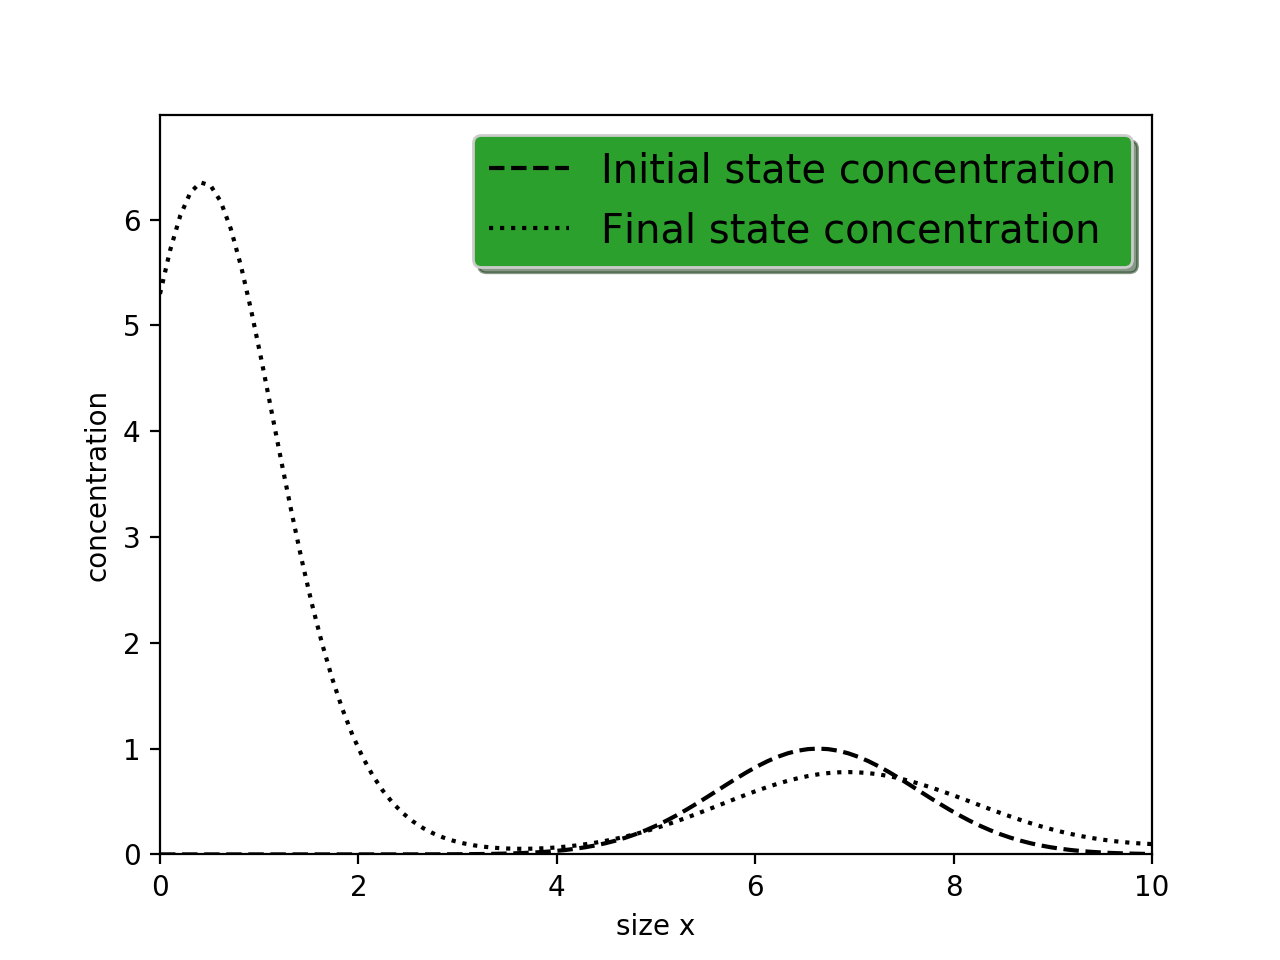
\includegraphics[width=7cm]{figures/state_if.png}
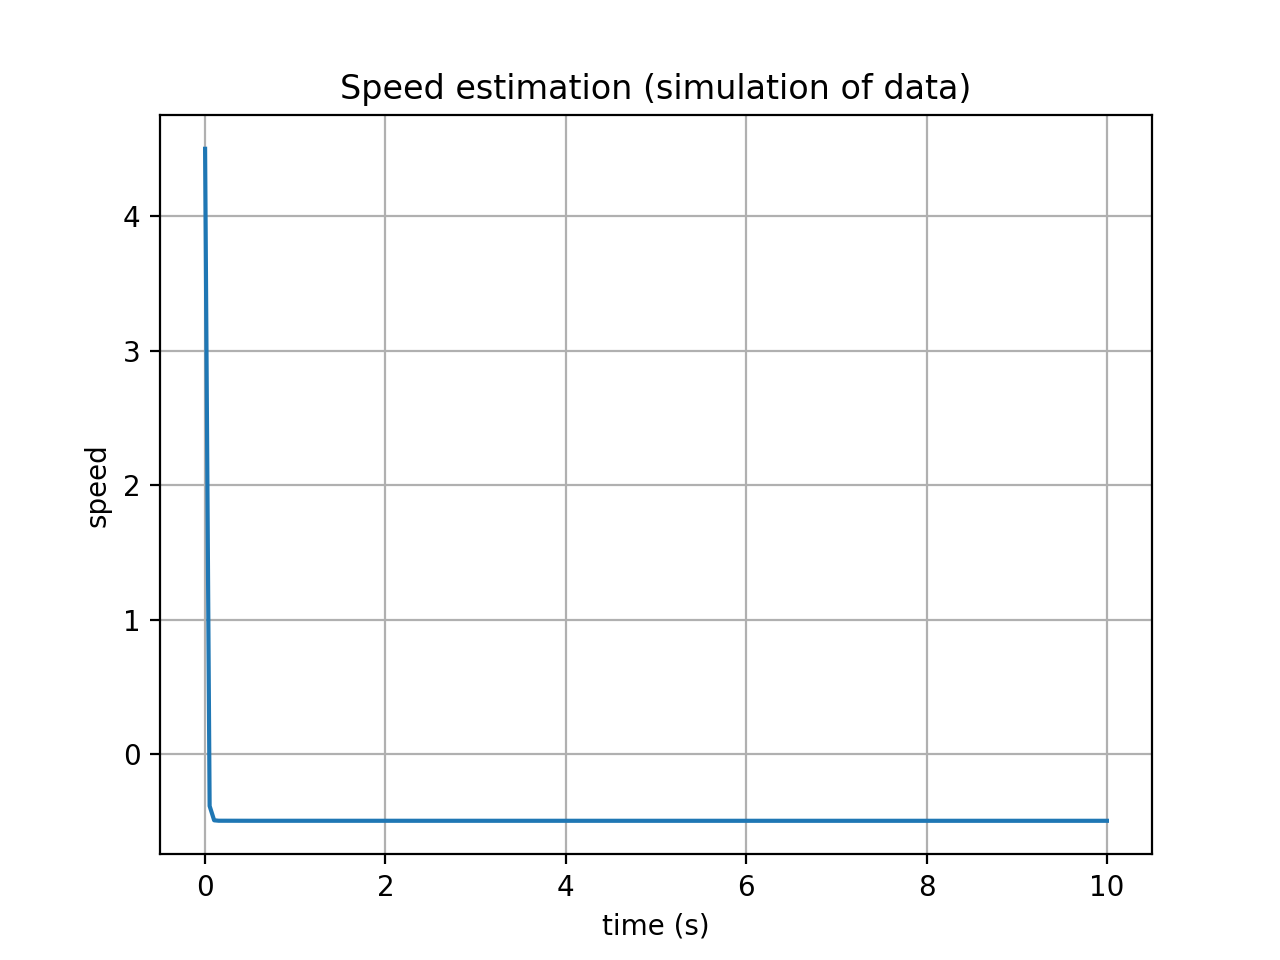
\includegraphics[width=7cm]{figures/Vitesse.png}

La simulation ci-dessous correspond à une dépolymérisation, et la vitesse v calculée est négative.

\section{Calcul de l'observateur}

\subsection{Calcul de $\zeta$}

Pour calculer $\zeta^j = \zeta(t_j) $, 
on discrétise l'équation ~\eqref{eq:tildez} 
par un schéma d'Euler explicite
sur le maillage $t_j = j\delta t$
et on obtient :
\[
\frac{\zeta^{j}-\zeta^{j-1}}{\delta t} = \lambda \zeta^{j} + \mu_1^j + \mu_2^j
\]

Soit :

\[
\zeta^{j+1} = \frac{1}{1-\lambda \delta t}(\zeta^{j-1} + \delta t \mu_1^j + \delta t \mu_2^j)
\]

\subsection{Calcul du noyau de convolution $k$}

D'après ce qui précède, on dispose à présent de la vitesse $v^j = v(j \delta t)$ pour l'équation de transport~\eqref{eq:general}. 
Il existe plussieurs façon de calculer $k$, par exemple pour la suite nous avons choisit d'utiliser la méthode des caractéristique
avec un pas de temps variable $\delta t = \delta x / v^j$. Les autres fonctions seront interpolées sur ce nouvel axe des temps. 
Cette résolution est robuste mais un peu trichée, en effet si $v$ est très grande ou très petite, le maillage est distordu.


Ainsi, il semblerait plus naturel d'utiliser sa formule explicite. Il suffit alors de déterminer $\theta(t) = \int_0^t v(s)ds $ puis d'interpoler $(x- \int_0^t v(s)ds)$ sur le maillage $ x_i =(i \delta x)$. Ce travail numérique est en cours.



\subsection{Convergence}

Afin d'optimiser le choix numérique du paramètre $\lambda$ 
et de s'assurer de la convergence de l'observateur.


On trace la différence entre la modélisation $\zeta^k$ et $Ty^k$ par exemple pour $\lambda = -0.1$.

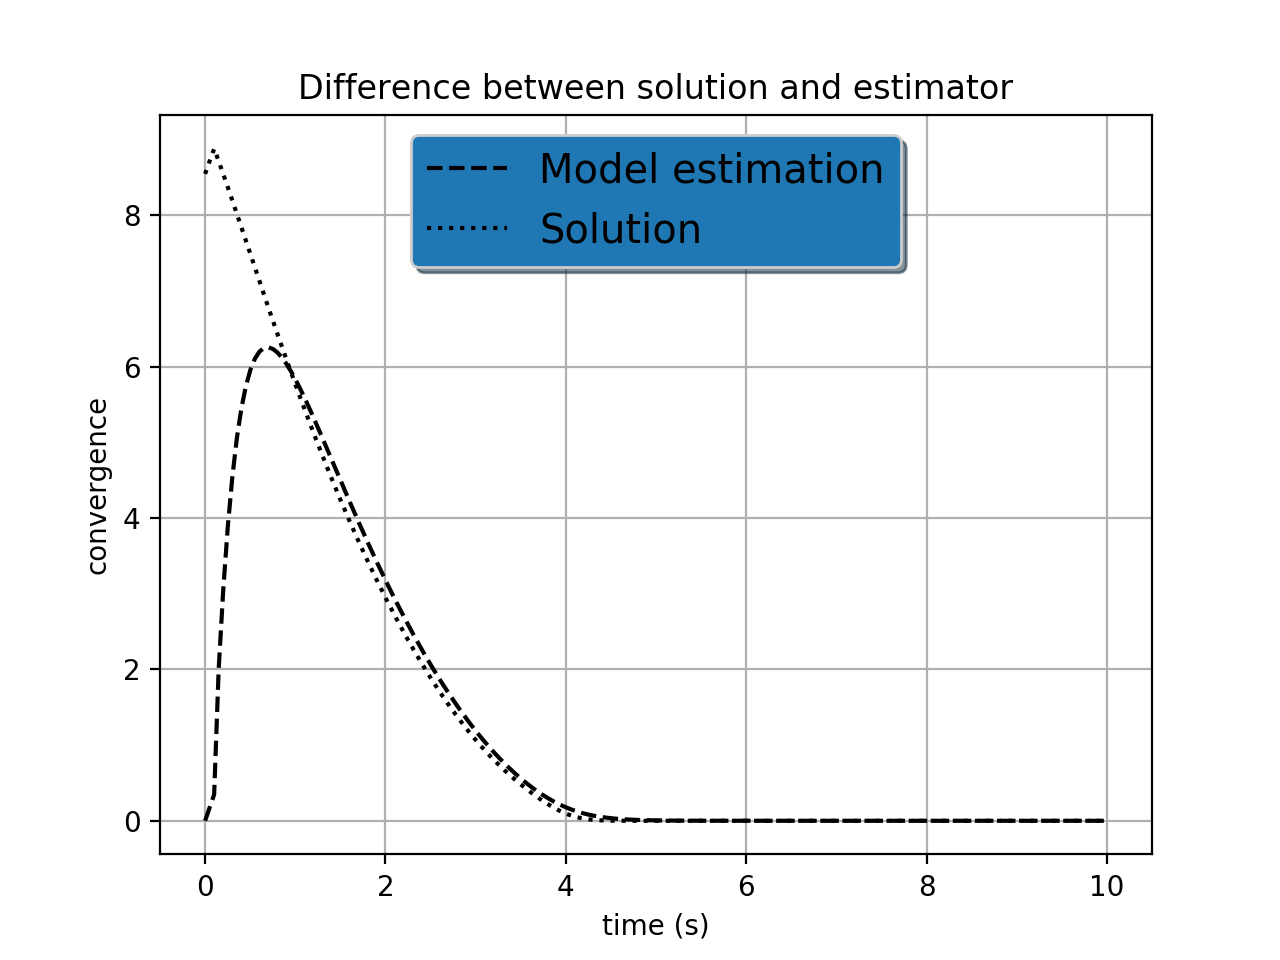
\includegraphics[width=9cm]{figures/Transformation.png}

On observe une convergence satisfaisante, 
et surtout elle survient avant que la masse des polymères aient entièrement dépolymérisé 
et que $y$ soit identiquement nul (ce qui nous qurqit empêché de reconstruire l'état).

Cependant, pour la suite, on préfèrera calculer l'état issu de l'équation de transport~\eqref{eq:general} 
par interpolation de $x- \int_0^t v(s)ds$ sur le maillage $ x_i =(i \delta x)$
et sa solution explicite $y(x,t) = y_0(x- \int_0^t v(s)ds)$.
Ce travail est en cours.

\section{Inversion de l'opérateur}

On dispose donc d'une série d'opérateurs $T_{\lambda}$ à inverser et pour un paramètre de régularisation $\alpha$. 

Pour résoudre ce problème d'optimisation, on peut avoir recours à la méthode de l'adjoint.

On définit pour la dynamique $y^{j+1} = F_j(y^j)$le Lagrangien discret : 

\[
\mathscr{L}(y,q) = \sum_j \delta t ((Ty)^j - \zeta^j)^2 
+ \alpha \sum_i \delta x (y_{0,i} - y_{\diamond,i})^2 
+ \sum_j \sum_i \delta x \delta t(y_i^{j+1} - (F_j(y^j))_i) q_i^j 
\]

Avec:

\[
(Ty)^j = \sum_i a_{i,j} y_i^j = A^j Y^j
\]

A l'optimum pour $(\bar{y},\bar{q})$ on a :

\[
\begin{split}
\langle \partial_y \mathscr{L}, \delta y \rangle_\mathscr{Y} &= 0\\
                                                             &= 2\sum_j \delta t (A^j Y^j - \zeta^j) A^j \delta y^j
															 + 2 \alpha \sum_i \delta x (y_{0,i} - y_{\diamond,i})
															 + \sum_j \sum_i \delta x \delta t
															 (\delta y_i^{j+1} -(F_j\delta y^j)_i) q_i^j \\
															 &= 2\sum_j \delta t (A^j Y^j - \zeta^j) A^j 
															 + 2 \alpha \sum_i \delta x (y_{0,i} - y_{\diamond,i})
															 -\sum_j \sum_i \delta x \delta t
															 \delta y_i^{j} q_i^{j-1}
															 - \sum_j \delta Y^j F_j^*Q^j
\end{split}
\]

Soit l'équation adjointe :

\[
Q^{j-1} + F_j^*Q^j = 2 \delta t (A^j Y^j - \zeta^j) A^j 
\]

Cette méthode doit être implémenter numériquement.


Une première solution serait donc de réaliser une optimisation pour chaque itération pour une suite $(\lambda_n)$ décroissante, 
en modifiant consécutivement l'apriori. 
Une deuxième serait de réaliser une optimisation globale et simultanée pour l'ensemble des $\lambda$.



%%%%%%%%%%%%%%%%%%%%%%%%%%%%%


   
%%%%%%%%%%%%%%%%%%%%%%%%%%%%%%%%%

\section{Conclusion}

			 

%%%%%%%%%%%%%%%%%%%%%%%%%%%%%%%%%%%%%%%%%%%%%%%%%%%%%%%%%%%%%%%%%%%%%%%%%%% REFERENCES

%%%%%%%%%%%%%%%%%%%%%%%%%%%%%%%%%%%%%%%%%%%%%%%%%%%%%%%%%%%%%%%%%%%%%%%%%%% REFERENCES

\medskip

\bibliographystyle{unsrt}%Used BibTeX style is unsrt
\bibliography{BIB20190110}

	
\end{document}
